\documentclass[10pt]{article}

\usepackage[a4paper,margin=0.9in]{geometry}
\usepackage{amsmath,amssymb}
\usepackage{booktabs}
\usepackage{longtable}
\usepackage{array}
\usepackage{tabularx}
\usepackage{graphicx}
\usepackage{caption}
\usepackage{float}
\usepackage{xcolor}
\usepackage[colorlinks=true,linkcolor=blue,citecolor=blue,urlcolor=blue]{hyperref}
\usepackage{titlesec}
\usepackage{fancyhdr}
\usepackage{parskip}

\graphicspath{{figures_v4/}{figures_osd462/}}
\newcommand{\gene}[1]{\textit{#1}}
\newcommand{\code}[1]{\texttt{#1}}

\pagestyle{fancy}
\fancyhf{}
\fancyhead[L]{\small Results \& Supplement --- Manuscript v8}
\fancyhead[R]{\small S\thepage}
\renewcommand{\headrulewidth}{0.4pt}
\renewcommand{\thepage}{S\arabic{page}}
\renewcommand{\thesection}{S\arabic{section}}
\renewcommand{\thetable}{S\arabic{table}}
\renewcommand{\thefigure}{S\arabic{figure}}

\title{\textbf{Results, Tables, and Supplementary Material}\\[0.3em]
\large Companion to Manuscript v8 --- A matrix-high / DCT-low kidney remodeling direction recurs across\\independent mouse spaceflight transcriptomes and aligns with the Cosmic Kidney Disease NCC phenotype}
\author{Ibrahim Shahid}
\date{Draft v8, May 2026}

\begin{document}
\maketitle
\thispagestyle{fancy}

\noindent
This document collects the full results tables, all figures, and supplementary material supporting Manuscript v8. It is organized to follow the manuscript's claim hierarchy: cohort design; the original within-RRRM-2 age-rewiring test; cross-cohort flight-vector recurrence; the matrix-high / DCT-low state; the live-return arm; mechanism context (OSD-253); and the pre-registered OSD-462 multi-omic anchor. All numbers were regenerated from the run artifacts \code{run\_20260519\_000547\_2500g} (transcriptomic) and \code{run\_20260521\_osd462\_anchor} (multi-omic anchor), and independently spot-verified against the raw OSD-462 workbooks.

\tableofcontents
\clearpage

% =====================================================================
\section{Pre-registration and hypothesis outcomes}

The OSD-462 multi-omic anchor was specified in a pre-registered plan (\path{docs/osd462_multiomics_analysis_plan.md}) with four hypotheses, each carrying an explicit falsification rule declared before any protein or phosphoprotein effect was computed. Table~\ref{tab:hyp} records the outcomes. Three hypotheses were falsified and one was strongly supported; under the pre-registration, every outcome --- including the nulls --- is a reportable result.

\begin{table}[H]
\centering\small
\caption{\textbf{Pre-registered hypotheses and outcomes for the OSD-462 multi-omic anchor.}}
\label{tab:hyp}
\begin{tabularx}{\textwidth}{>{\bfseries}p{0.06\textwidth}X p{0.16\textwidth}}
\toprule
ID & Hypothesis and pre-registered prediction & Outcome \\
\midrule
H1 & Matrix/ECM transcripts and proteins are concordant in flight (matrix proteins up; concordance exceeds matched null). & \textbf{Falsified.} Matrix proteins moved opposite transcripts. \\
H2 & DCT/NCC-WNK transcripts and proteins are concordant (transporter proteins down; concordance exceeds null). & \textbf{Falsified.} No protein-abundance effect; total NCC protein flat. \\
H3 & The WNK--SPAK/OSR1--NCC phospho-axis is suppressed in flight. & \textbf{Supported.} NCC activating cluster and SPAK strongly down. \\
H4 & RRRM-2 LIONESS/node2vec network candidates are enriched for OSD-462 protein- or phosphoprotein-changing genes. & \textbf{Falsified.} No enrichment ($p\geq0.23$). \\
\bottomrule
\end{tabularx}
\end{table}

\noindent
\textbf{Decision-table outcome.} Protein-abundance concordance was null for both matrix and DCT gene sets; the DCT signal relocated to the phospho/activity layer. Per the pre-registered claim ceiling, the result is a molecular claim (transcript- and signaling-level), with histology and urine/serum chemistry remaining out of scope and explicitly future work.

% =====================================================================
\section{Cohort design}

\begin{table}[H]
\centering\small
\caption{\textbf{Cohorts analyzed.} RRRM-2 is the factorial bridge; OSD-513 and OSD-253 are independent transcriptomic cohorts; OSD-462 (RR-10) is the multi-omic anchor and the source of the Cosmic Kidney Disease mouse kidney phosphoproteomics.}
\label{tab:cohorts}
\begin{tabularx}{\textwidth}{l l l l X}
\toprule
Cohort & Accession & Tissue / sex & Modalities & Role \\
\midrule
RRRM-2 & OSD-771 & Kidney / female & RNA-seq & Factorial bridge: Age $\times$ Arm (ISS-T, LAR) $\times$ Flight, $n=5$/cell \\
OSD-513 & OSD-513 & Kidney / -- & RNA-seq & Independent flight-vector recurrence cohort \\
OSD-253 & OSD-253 & Kidney / -- & RNA-seq & Strain/mechanism context (C57BL/6J vs C3H/HeJ) \\
OSD-462 & OSD-462 (RR-10) & Kidney / female & RNA-seq, proteomics, phosphoproteomics & Multi-omic anchor; Cosmic Kidney Disease mouse cohort \\
Tabula Muris Senis & --- & Kidney & scRNA-seq & External aging reference \\
\bottomrule
\end{tabularx}
\end{table}

% =====================================================================
\section{Within-RRRM-2 age-vector stability (original claim, not supported)}

\begin{table}[H]
\centering\small
\caption{\textbf{Bootstrap angular stability of RRRM-2 control-aging vectors.} Module and pathway are the primary biological resolutions; three of four arm-resolution settings failed the stability gate, so the original within-cohort age-rewiring contrast is not promoted as a claim.}
\label{tab:stab}
\begin{tabular}{llrrrrc}
\toprule
Arm & Resolution & Full norm & Median cosine & Lower CI & Required lower & Passed \\
\midrule
ISS-T & pathway & 0.167 & 0.787 & 0.248 & 0.400 & no \\
ISS-T & module & 0.325 & 0.750 & 0.056 & 0.400 & no \\
ISS-T & gene & 10.152 & 0.746 & 0.545 & 0.200 & yes \\
ISS-T & LIONESS-node & 10.152 & 0.745 & 0.549 & 0.200 & yes \\
LAR & pathway & 0.221 & 0.890 & 0.345 & 0.400 & no \\
LAR & module & 0.353 & 0.774 & 0.493 & 0.400 & yes \\
LAR & gene & 9.687 & 0.742 & 0.563 & 0.200 & yes \\
LAR & LIONESS-node & 9.687 & 0.737 & 0.556 & 0.200 & yes \\
\bottomrule
\end{tabular}
\end{table}

% =====================================================================
\section{Cross-OSDR flight-vector recurrence}

\begin{table}[H]
\centering\small
\caption{\textbf{Cross-OSDR pathway-vector alignment.} OSD-513 is interpreted as directional recurrence; OSD-253 as context. $p_{\mathrm{perm}}$ is the directional external-label permutation sensitivity with the RRRM-2 reference vector held fixed.}
\label{tab:cross}
\begin{tabular}{lllrrrrr}
\toprule
Study & Scenario & Arm & Point & Median & Lower CI & Upper CI & $p_{\mathrm{perm}}$ \\
\midrule
OSD-513 & powered HGC & ISS-T & 0.641 & 0.625 & 0.351 & 0.814 & 0.127 \\
OSD-513 & powered HGC & LAR & $-0.511$ & $-0.498$ & $-0.726$ & $-0.231$ & 0.178 \\
OSD-253 & original GC & ISS-T & 0.674 & 0.602 & $-0.411$ & 0.836 & 0.141 \\
OSD-253 & original GC & LAR & $-0.679$ & $-0.608$ & $-0.816$ & 0.415 & 0.125 \\
OSD-253 & rerun GC & ISS-T & 0.474 & 0.470 & $-0.040$ & 0.688 & 0.269 \\
OSD-253 & rerun GC & LAR & $-0.318$ & $-0.309$ & $-0.572$ & 0.183 & 0.344 \\
\bottomrule
\end{tabular}
\end{table}

\begin{table}[H]
\centering\small
\caption{\textbf{Pathway construction of the recurrent ISS-T remodeling axis.} Effects are pathway-scale FLT-minus-GC contrasts; the axis is oriented so ECM/fibrosis is positive and DCT/NCC-WNK suppression is negative.}
\label{tab:axis}
\begin{tabular}{lrrrc}
\toprule
Pathway & RRRM-2 ISS-T & OSD-513 & Axis weight & Primary axis \\
\midrule
ECM remodeling & 0.949 & 0.801 & 0.622 & yes \\
Fibrosis & 0.764 & 0.652 & 0.504 & yes \\
DCT/NCC-WNK & $-0.398$ & $-0.889$ & $-0.452$ & yes \\
Apoptosis & 0.674 & 0.386 & 0.378 & yes \\
Oxidative stress & 0.198 & 0.104 & 0.108 & yes \\
Inflammation & 0.561 & $-0.092$ & 0.000 & no \\
Ion transport & 0.329 & $-0.762$ & 0.000 & sensitivity \\
Lipid metabolism & $-0.320$ & 0.156 & 0.000 & no \\
Calcium handling & 0.003 & $-0.550$ & 0.000 & no \\
\bottomrule
\end{tabular}
\end{table}

% =====================================================================
\section{Matrix-high / DCT-low state and live-return arm}

\begin{table}[H]
\centering\small
\caption{\textbf{State-space component effects (FLT-minus-GC) and arm-by-flight interactions.} Young LAR effects are shown to be underpowered and not statistically distinguishable from zero.}
\label{tab:state}
\begin{tabular}{llrrr}
\toprule
Component & Arm / scope & Effect & Welch $p$ / interaction $p$ & BH $q$ \\
\midrule
matrix-minus-DCT & ISS-T pooled & $+2.254$ & 0.003 & 0.020 \\
matrix-minus-DCT & LAR pooled & $-0.112$ & 0.865 & 0.895 \\
matrix-minus-DCT & ISS-T young & $+3.204$ & 0.005 & 0.025 \\
matrix-minus-DCT & LAR young & $-0.782$ & 0.361 & 0.542 \\
matrix-minus-DCT & Arm$\times$Flight interaction & $+2.366$ & 0.016 & 0.027 \\
matrix component & Arm$\times$Flight interaction & $+1.738$ & --- & 0.004 \\
DCT transport & Arm$\times$Flight interaction & $-0.628$ & --- & 0.344 \\
mechanism-score vector & cos(LAR, ISS-T) pooled & $-0.725$ & CI $[-0.874,-0.122]$ & --- \\
\bottomrule
\end{tabular}
\end{table}

% =====================================================================
\section{OSD-462 multi-omic anchor}

\subsection{RNA recurrence gate (Layer 4)}

The OSD-462 Space~Flight minus Ground~Control RNA pathway vector reproduced the RRRM-2 ISS-T matrix-high / DCT-low direction with cosine $0.869$ (95\% bootstrap CI $0.648$--$0.903$; bootstrap median $0.823$) across 11 pathways; leave-one-pathway-out cosine ranged $0.823$--$0.904$. The recurrence gate passed.

\begin{table}[H]
\centering\small
\caption{\textbf{OSD-462 RNA pathway flight effects vs RRRM-2 ISS-T.} Space~Flight minus Ground~Control (OSD-462) and FLT-minus-GC (RRRM-2 ISS-T).}
\label{tab:rnapath}
\begin{tabular}{lrrc}
\toprule
Pathway & OSD-462 RNA effect & RRRM-2 ISS-T effect & Sign agreement \\
\midrule
ecm\_organization & 0.222 & 0.280 & 1.000 \\
fibrosis\_tgfb\_emt & 0.149 & 0.025 & 1.000 \\
tlr4\_innate & 0.075 & 0.095 & 1.000 \\
integrin\_cell\_adhesion & 0.119 & 0.087 & 1.000 \\
s1p\_s1pr3 & 0.123 & 0.106 & 1.000 \\
mmp\_adam\_proteolysis & 0.197 & 0.123 & 1.000 \\
dct\_ncc\_wnk\_transport & -0.130 & -0.075 & 1.000 \\
tubular\_transport\_broad & -0.048 & 0.042 & 0.000 \\
oxidative\_stress\_nrf2 & 0.021 & 0.005 & 1.000 \\
macrophage\_inflammation & 0.109 & 0.090 & 1.000 \\
preservation\_stress\_response & 0.157 & 0.293 & 1.000 \\
\bottomrule
\end{tabular}
\end{table}

\subsection{Protein-abundance concordance (Layer 1)}

Genome-wide RRRM-2-RNA versus OSD-462-protein flight-effect correlation was negligible (Spearman $0.043$). No targeted gene set was concordant in its predicted direction against the abundance- and peptide-matched random-gene-set null. The matrix/ECM set moved opposite its transcripts.

\begin{table}[H]
\centering\small
\caption{\textbf{OSD-462 protein-abundance concordance by gene set.} Signed mean protein flight effect with the matched random-gene-set null interval. No set is concordant in its predicted direction.}
\label{tab:protconc}
\begin{tabular}{llrlrl}
\toprule
Gene set & Kind & $n$ & Predicted dir. & Signed mean effect & Matched-null interval \\
\midrule
dct\_ncc\_wnk\_transport & family & 10 & down & -0.044 & [-0.052, 0.047] \\
ecm\_organization & family & 15 & up & -0.107 & [-0.082, 0.056] \\
tlr4\_innate & family & 8 & up & -0.021 & [-0.040, 0.031] \\
s1p\_s1pr3 & family & 9 & up & -0.045 & [-0.055, 0.054] \\
tubular\_transport\_broad & control & 15 & up & 0.043 & [-0.061, 0.060] \\
\bottomrule
\end{tabular}
\end{table}

\subsection{WNK--SPAK/OSR1--NCC phospho-axis (Layer 2)}

The phosphoproteomics checkpoint passed (all targeted NCC, SPAK, OSR1, WNK sites quantified). Total NCC protein abundance was unchanged in flight ($+0.089$), so phosphosite changes reflect altered phosphorylation stoichiometry. Table~\ref{tab:phosphofull} lists every quantified phosphosite on the WNK--SPAK/OSR1--NCC chain. The NCC N-terminal regulatory (SPAK/OSR1-target) cluster and SPAK sites are strongly suppressed; non-regulatory NCC sites are unchanged --- an internal negative control against a global normalization artifact.

\begin{longtable}{lllrrrrr}
\caption{\textbf{Complete OSD-462 WNK--SPAK/OSR1--NCC phosphosite flight effects.} Space~Flight minus Ground~Control, log$_2$ scale, plex-corrected. $n$ is FL/GC channels.}\label{tab:phosphofull}\\
\toprule
Gene & Site & Kind & $n$ & Effect & CI low & CI high & $p$ value \\
\midrule
\endfirsthead
\multicolumn{8}{l}{\small\itshape Table S\arabic{table} continued}\\
\toprule
Gene & Site & Kind & $n$ & Effect & CI low & CI high & $p$ value \\
\midrule
\endhead
\bottomrule
\endfoot
Calb1 & 60 & single & 5/5 & 0.177 & -0.016 & 0.370 & 0.067 \\
Cul3 & 737 & single & 10/10 & 0.121 & -4.8e-04 & 0.243 & 0.051 \\
Nedd4l & 331 & single & 5/5 & 0.077 & -0.223 & 0.378 & 0.570 \\
Nedd4l & 332 & single & 10/10 & 0.002 & -0.069 & 0.073 & 0.955 \\
Nedd4l & 373 & single & 10/10 & -0.230 & -0.440 & -0.021 & 0.033 \\
Nedd4l & 480 & single & 10/10 & -0.264 & -0.383 & -0.144 & 2.4e-04 \\
Nedd4l & 484 & single & 5/5 & -0.412 & -0.637 & -0.186 & 0.003 \\
Nedd4l & 504 & single & 10/10 & 0.040 & -0.106 & 0.186 & 0.573 \\
Oxsr1 & 339 & single & 10/10 & 0.005 & -0.055 & 0.065 & 0.867 \\
Sgk1 & 494 & single & 10/10 & -0.114 & -0.683 & 0.454 & 0.677 \\
Slc12a3 & 120 & single & 10/10 & 0.027 & -0.175 & 0.229 & 0.780 \\
Slc12a3 & 120;122 & composite & 10/10 & 0.191 & -0.046 & 0.429 & 0.107 \\
Slc12a3 & 120;124 & composite & 10/10 & 0.039 & -0.164 & 0.243 & 0.688 \\
Slc12a3 & 122 & single & 10/10 & 0.045 & -0.168 & 0.257 & 0.665 \\
Slc12a3 & 122;124 & composite & 10/10 & 0.168 & -0.062 & 0.399 & 0.141 \\
Slc12a3 & 124 & single & 10/10 & 0.051 & -0.254 & 0.357 & 0.727 \\
Slc12a3 & 53 & single & 10/10 & -0.851 & -1.257 & -0.445 & 3.8e-04 \\
Slc12a3 & 53;65 & composite & 10/10 & -0.350 & -0.496 & -0.204 & 9.7e-05 \\
Slc12a3 & 53;68 & composite & 5/5 & -0.133 & -0.758 & 0.493 & 0.638 \\
Slc12a3 & 56;65 & composite & 5/5 & -0.124 & -0.560 & 0.312 & 0.530 \\
Slc12a3 & 58;65 & composite & 10/10 & -0.545 & -0.836 & -0.254 & 0.001 \\
Slc12a3 & 65 & single & 10/10 & -0.790 & -1.038 & -0.543 & 3.5e-06 \\
Slc12a3 & 65;68 & composite & 10/10 & -1.563 & -2.005 & -1.121 & 9.3e-07 \\
Slc12a3 & 68 & single & 10/10 & -0.794 & -1.168 & -0.420 & 3.3e-04 \\
Slc12a3 & 89 & single & 10/10 & -0.930 & -1.305 & -0.556 & 6.6e-05 \\
Slc12a3 & 96 & single & 10/10 & 0.048 & -0.092 & 0.189 & 0.480 \\
Stk39 & 366 & single & 10/10 & -0.520 & -0.706 & -0.334 & 1.7e-05 \\
Stk39 & 382 & single & 5/5 & -0.829 & -1.768 & 0.109 & 0.076 \\
Stk39 & 382;383 & composite & 10/10 & -0.368 & -0.579 & -0.157 & 0.002 \\
Stk39 & 383 & single & 10/10 & -0.793 & -1.160 & -0.426 & 2.8e-04 \\
Stk39 & 397 & single & 10/10 & 0.073 & -0.013 & 0.159 & 0.092 \\
Wnk1 & 157 & single & 5/5 & -0.129 & -0.346 & 0.087 & 0.206 \\
Wnk1 & 17 & single & 10/10 & -0.159 & -0.335 & 0.018 & 0.075 \\
Wnk1 & 172 & single & 10/10 & 0.014 & -0.128 & 0.156 & 0.834 \\
Wnk1 & 185 & single & 5/5 & 0.008 & -0.252 & 0.269 & 0.942 \\
Wnk1 & 2258 & single & 10/10 & -0.200 & -0.482 & 0.083 & 0.154 \\
Wnk1 & 2280;2282 & composite & 5/5 & -0.121 & -0.592 & 0.350 & 0.569 \\
Wnk1 & 2280;2282;2285 & composite & 10/10 & 0.129 & -0.017 & 0.275 & 0.080 \\
Wnk1 & 2282;2285 & composite & 10/10 & 0.135 & -0.120 & 0.390 & 0.280 \\
Wnk1 & 2285 & single & 5/5 & 0.022 & -0.467 & 0.510 & 0.921 \\
Wnk1 & 2392 & single & 5/5 & -0.628 & -0.880 & -0.376 & 4.4e-04 \\
Wnk1 & 2623 & single & 5/5 & -0.297 & -0.563 & -0.030 & 0.033 \\
Wnk1 & 2625 & single & 10/10 & -0.362 & -0.609 & -0.114 & 0.007 \\
Wnk4 & 1014 & single & 10/10 & -0.036 & -0.096 & 0.024 & 0.217 \\
Wnk4 & 1025 & single & 10/10 & 0.190 & 0.051 & 0.329 & 0.010 \\
Wnk4 & 1025;1033 & composite & 10/10 & 0.287 & 0.093 & 0.481 & 0.006 \\
Wnk4 & 1033 & single & 10/10 & 0.290 & 0.097 & 0.484 & 0.006 \\
Wnk4 & 125 & single & 10/10 & -0.049 & -0.273 & 0.175 & 0.649 \\
Wnk4 & 639 & single & 5/5 & -0.110 & -0.465 & 0.246 & 0.496 \\
Wnk4 & 783 & single & 5/5 & 0.118 & -0.033 & 0.269 & 0.110 \\
Wnk4 & 95 & single & 10/10 & -0.006 & -0.075 & 0.063 & 0.861 \\
\end{longtable}

\subsection{Network-candidate translation (Layer 3)}

RRRM-2 LIONESS/node2vec top-composite candidates were not enriched among OSD-462 protein-changing genes at any top-$k$ threshold.

\begin{table}[H]
\centering\small
\caption{\textbf{Network-candidate translation to OSD-462 proteins.} Enrichment of RRRM-2 network-prioritized genes among protein-changing genes vs the matched null.}
\label{tab:network}
\begin{tabular}{rrrrr}
\toprule
Top $k$ & Candidates w/ protein & Mean $|$effect$|$ & Null median & Enrichment $p$ \\
\midrule
25 & 14 & 0.103 & 0.081 & 0.227 \\
50 & 22 & 0.088 & 0.079 & 0.329 \\
100 & 41 & 0.089 & 0.080 & 0.298 \\
\bottomrule
\end{tabular}
\end{table}

% =====================================================================
\section{Figures}

\begin{figure}[H]
\centering
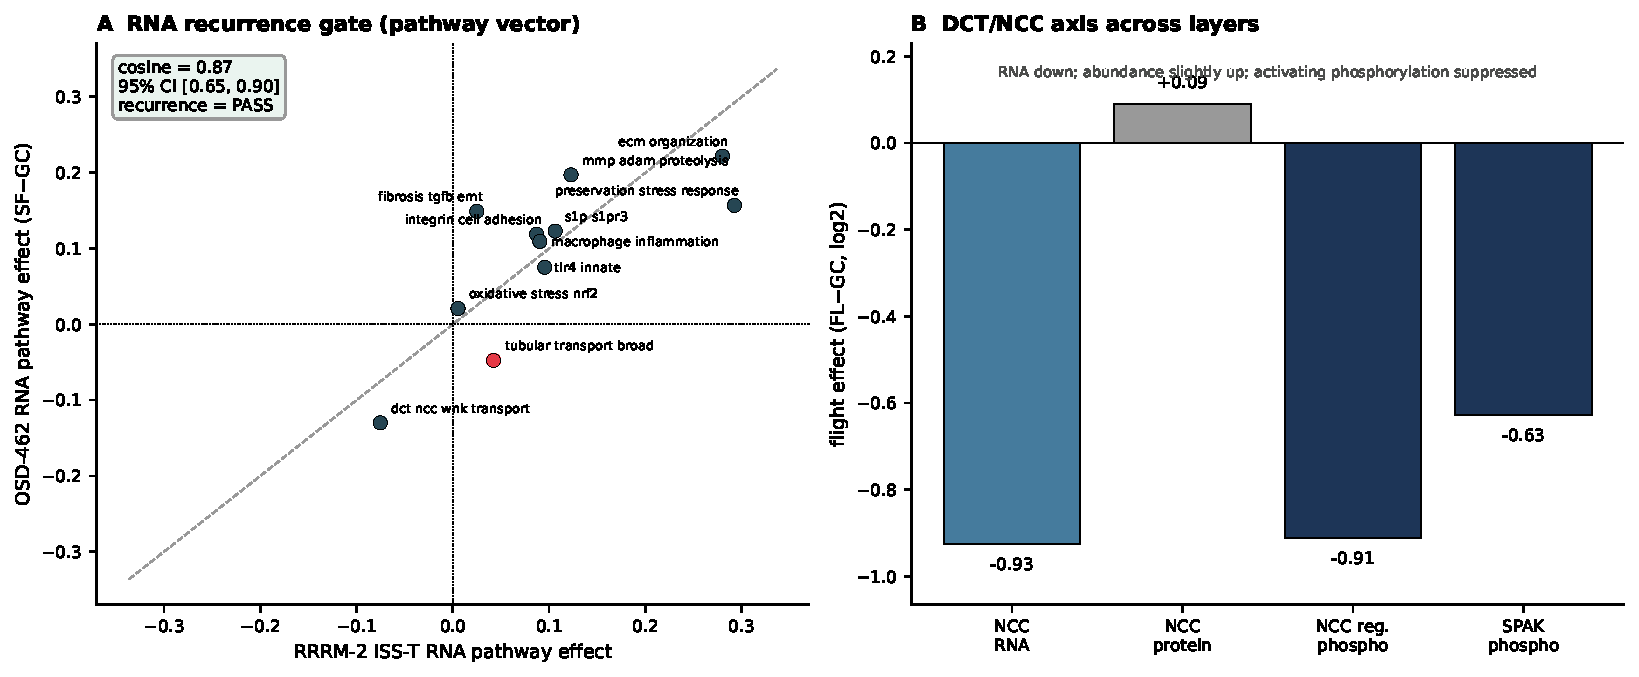
\includegraphics[width=0.9\textwidth]{fig_osd462_rna_recurrence.pdf}
\caption{\textbf{OSD-462 RNA recurrence gate.} The OSD-462 Space~Flight minus Ground~Control RNA pathway vector reproduces the RRRM-2 ISS-T matrix-high / DCT-low direction (cosine $0.87$, 95\% CI $0.65$--$0.90$), with leave-one-pathway-out stability.}
\end{figure}

\begin{figure}[H]
\centering
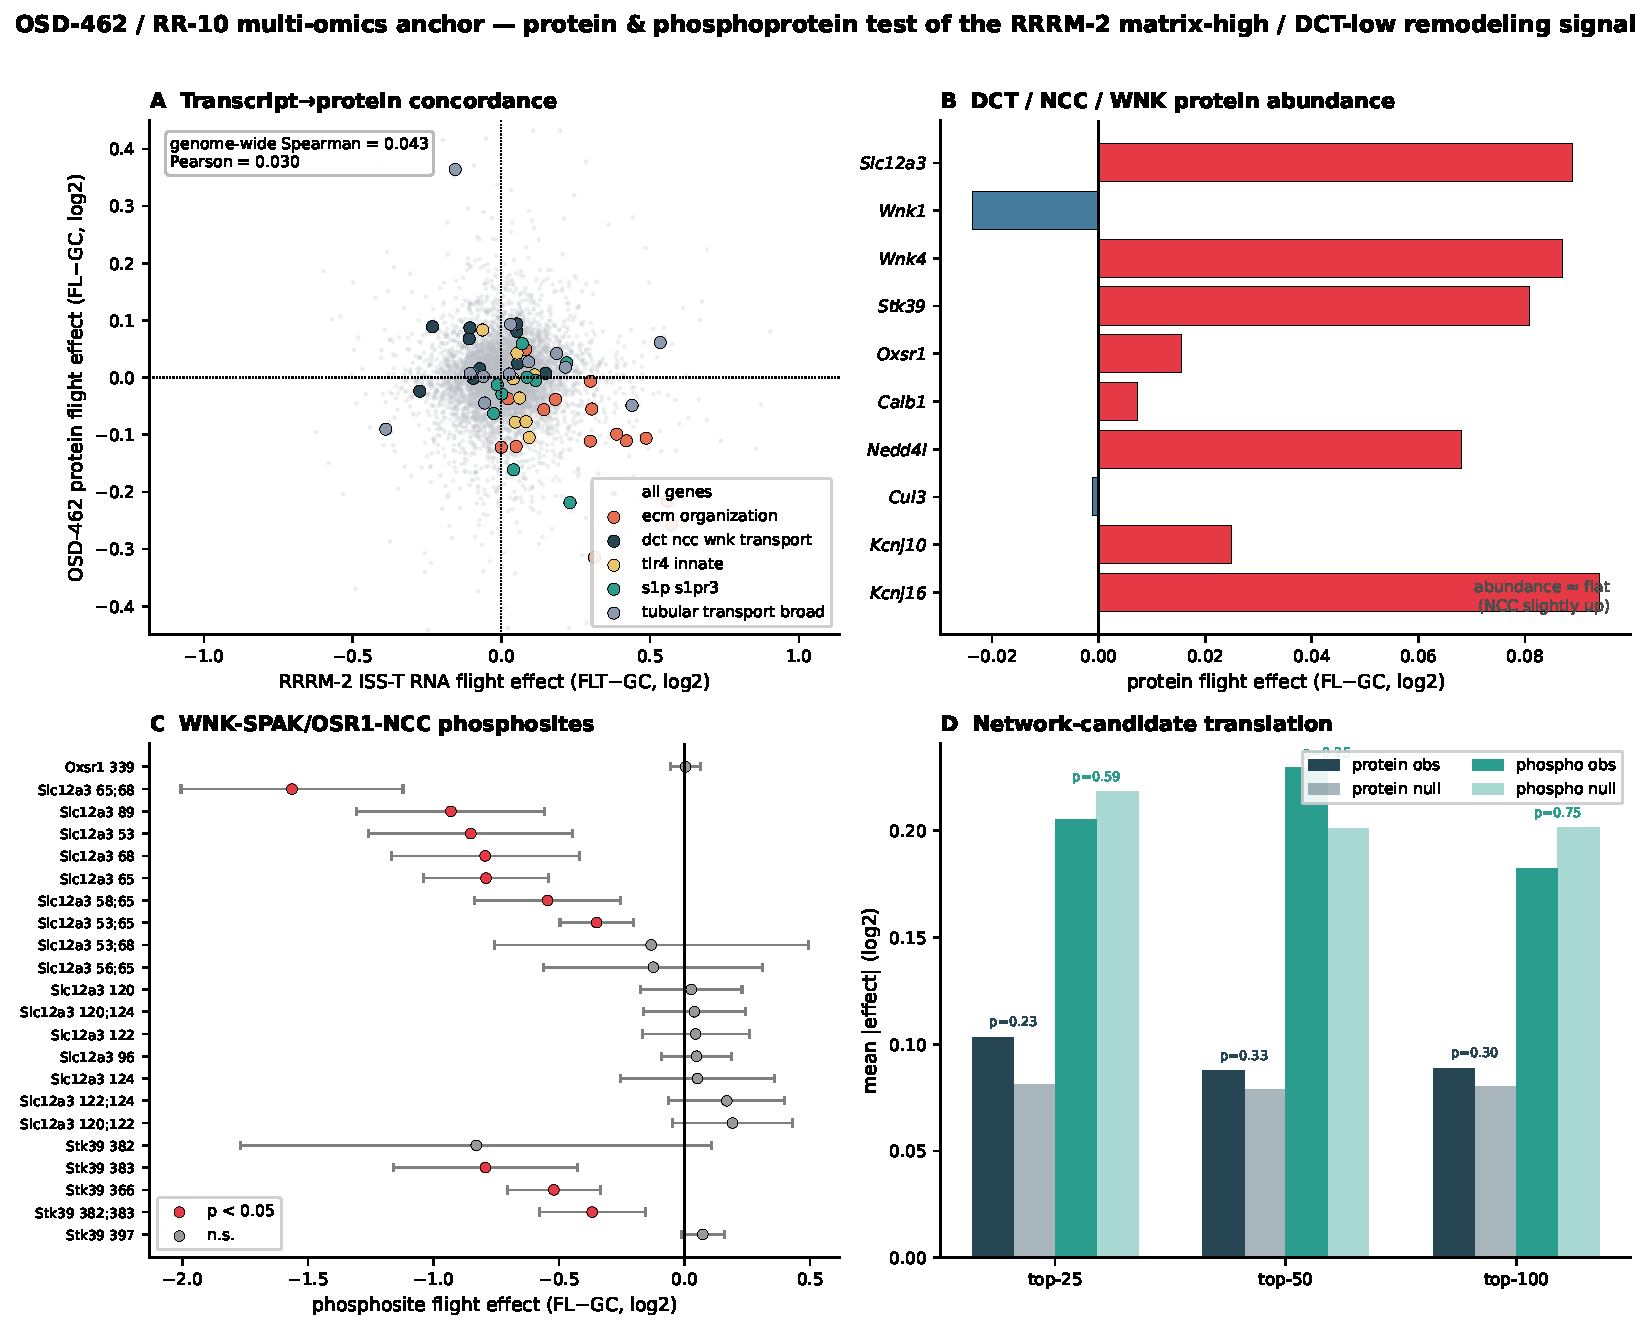
\includegraphics[width=\textwidth]{fig_osd462_multiomics_dashboard.pdf}
\caption{\textbf{OSD-462 multi-omic anchor dashboard.} Transcript-level recurrence, protein-abundance null, and phospho-axis suppression of the WNK--SPAK/OSR1--NCC activating cluster.}
\end{figure}

\begin{figure}[H]
\centering
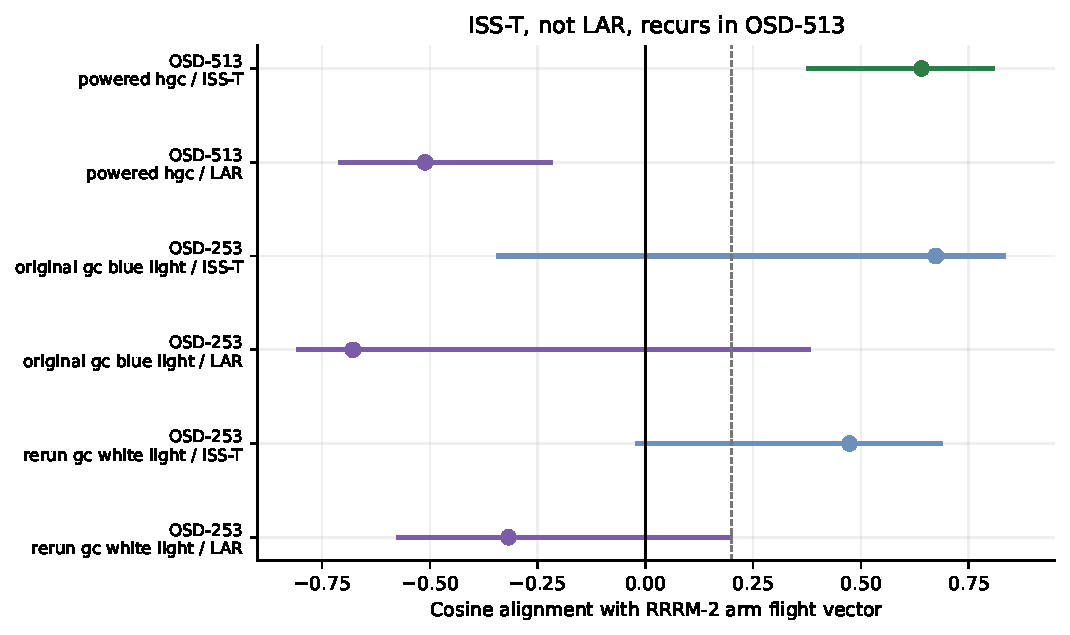
\includegraphics[width=\textwidth]{fig3_cross_osdr_alignment.pdf}
\caption{\textbf{Cross-OSDR pathway-vector alignment.} RRRM-2 ISS-T aligns with OSD-513; LAR anti-aligns directionally.}
\end{figure}

\begin{figure}[H]
\centering
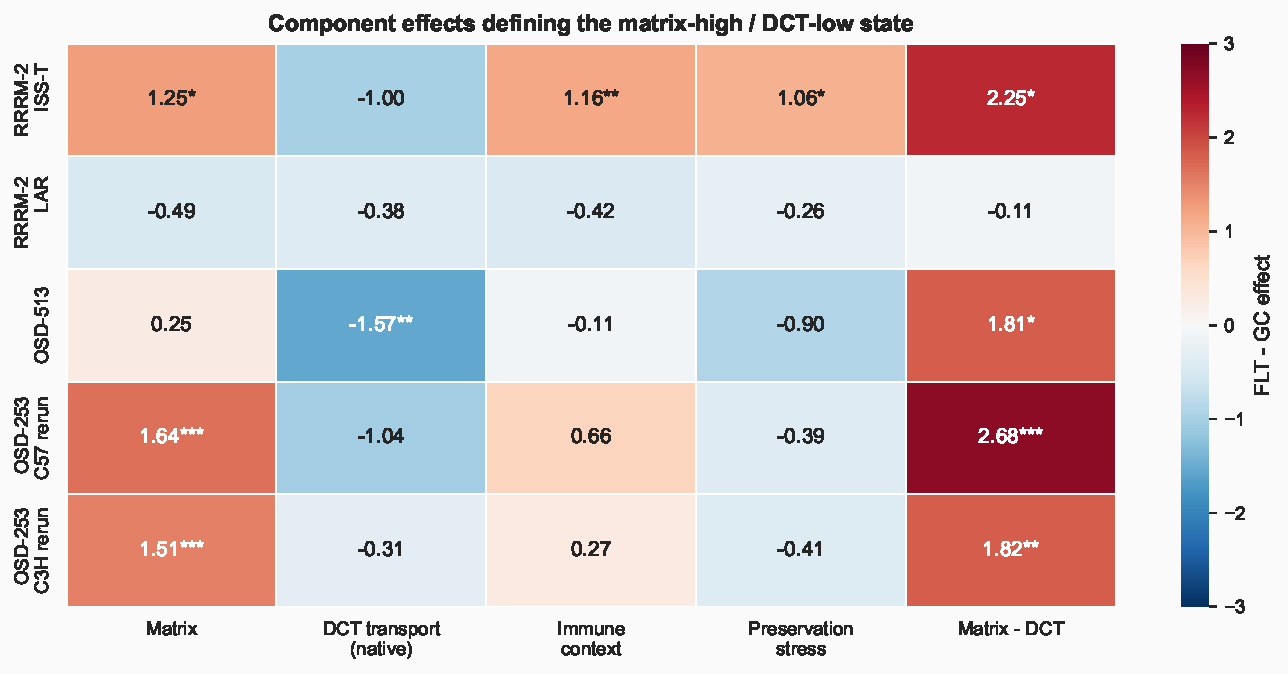
\includegraphics[width=\textwidth]{fig11_state_component_effects.pdf}
\caption{\textbf{Matrix-high / DCT-low state component effects.} FLT-minus-GC effects in standardized component units; DCT transport in native direction.}
\end{figure}

\begin{figure}[H]
\centering
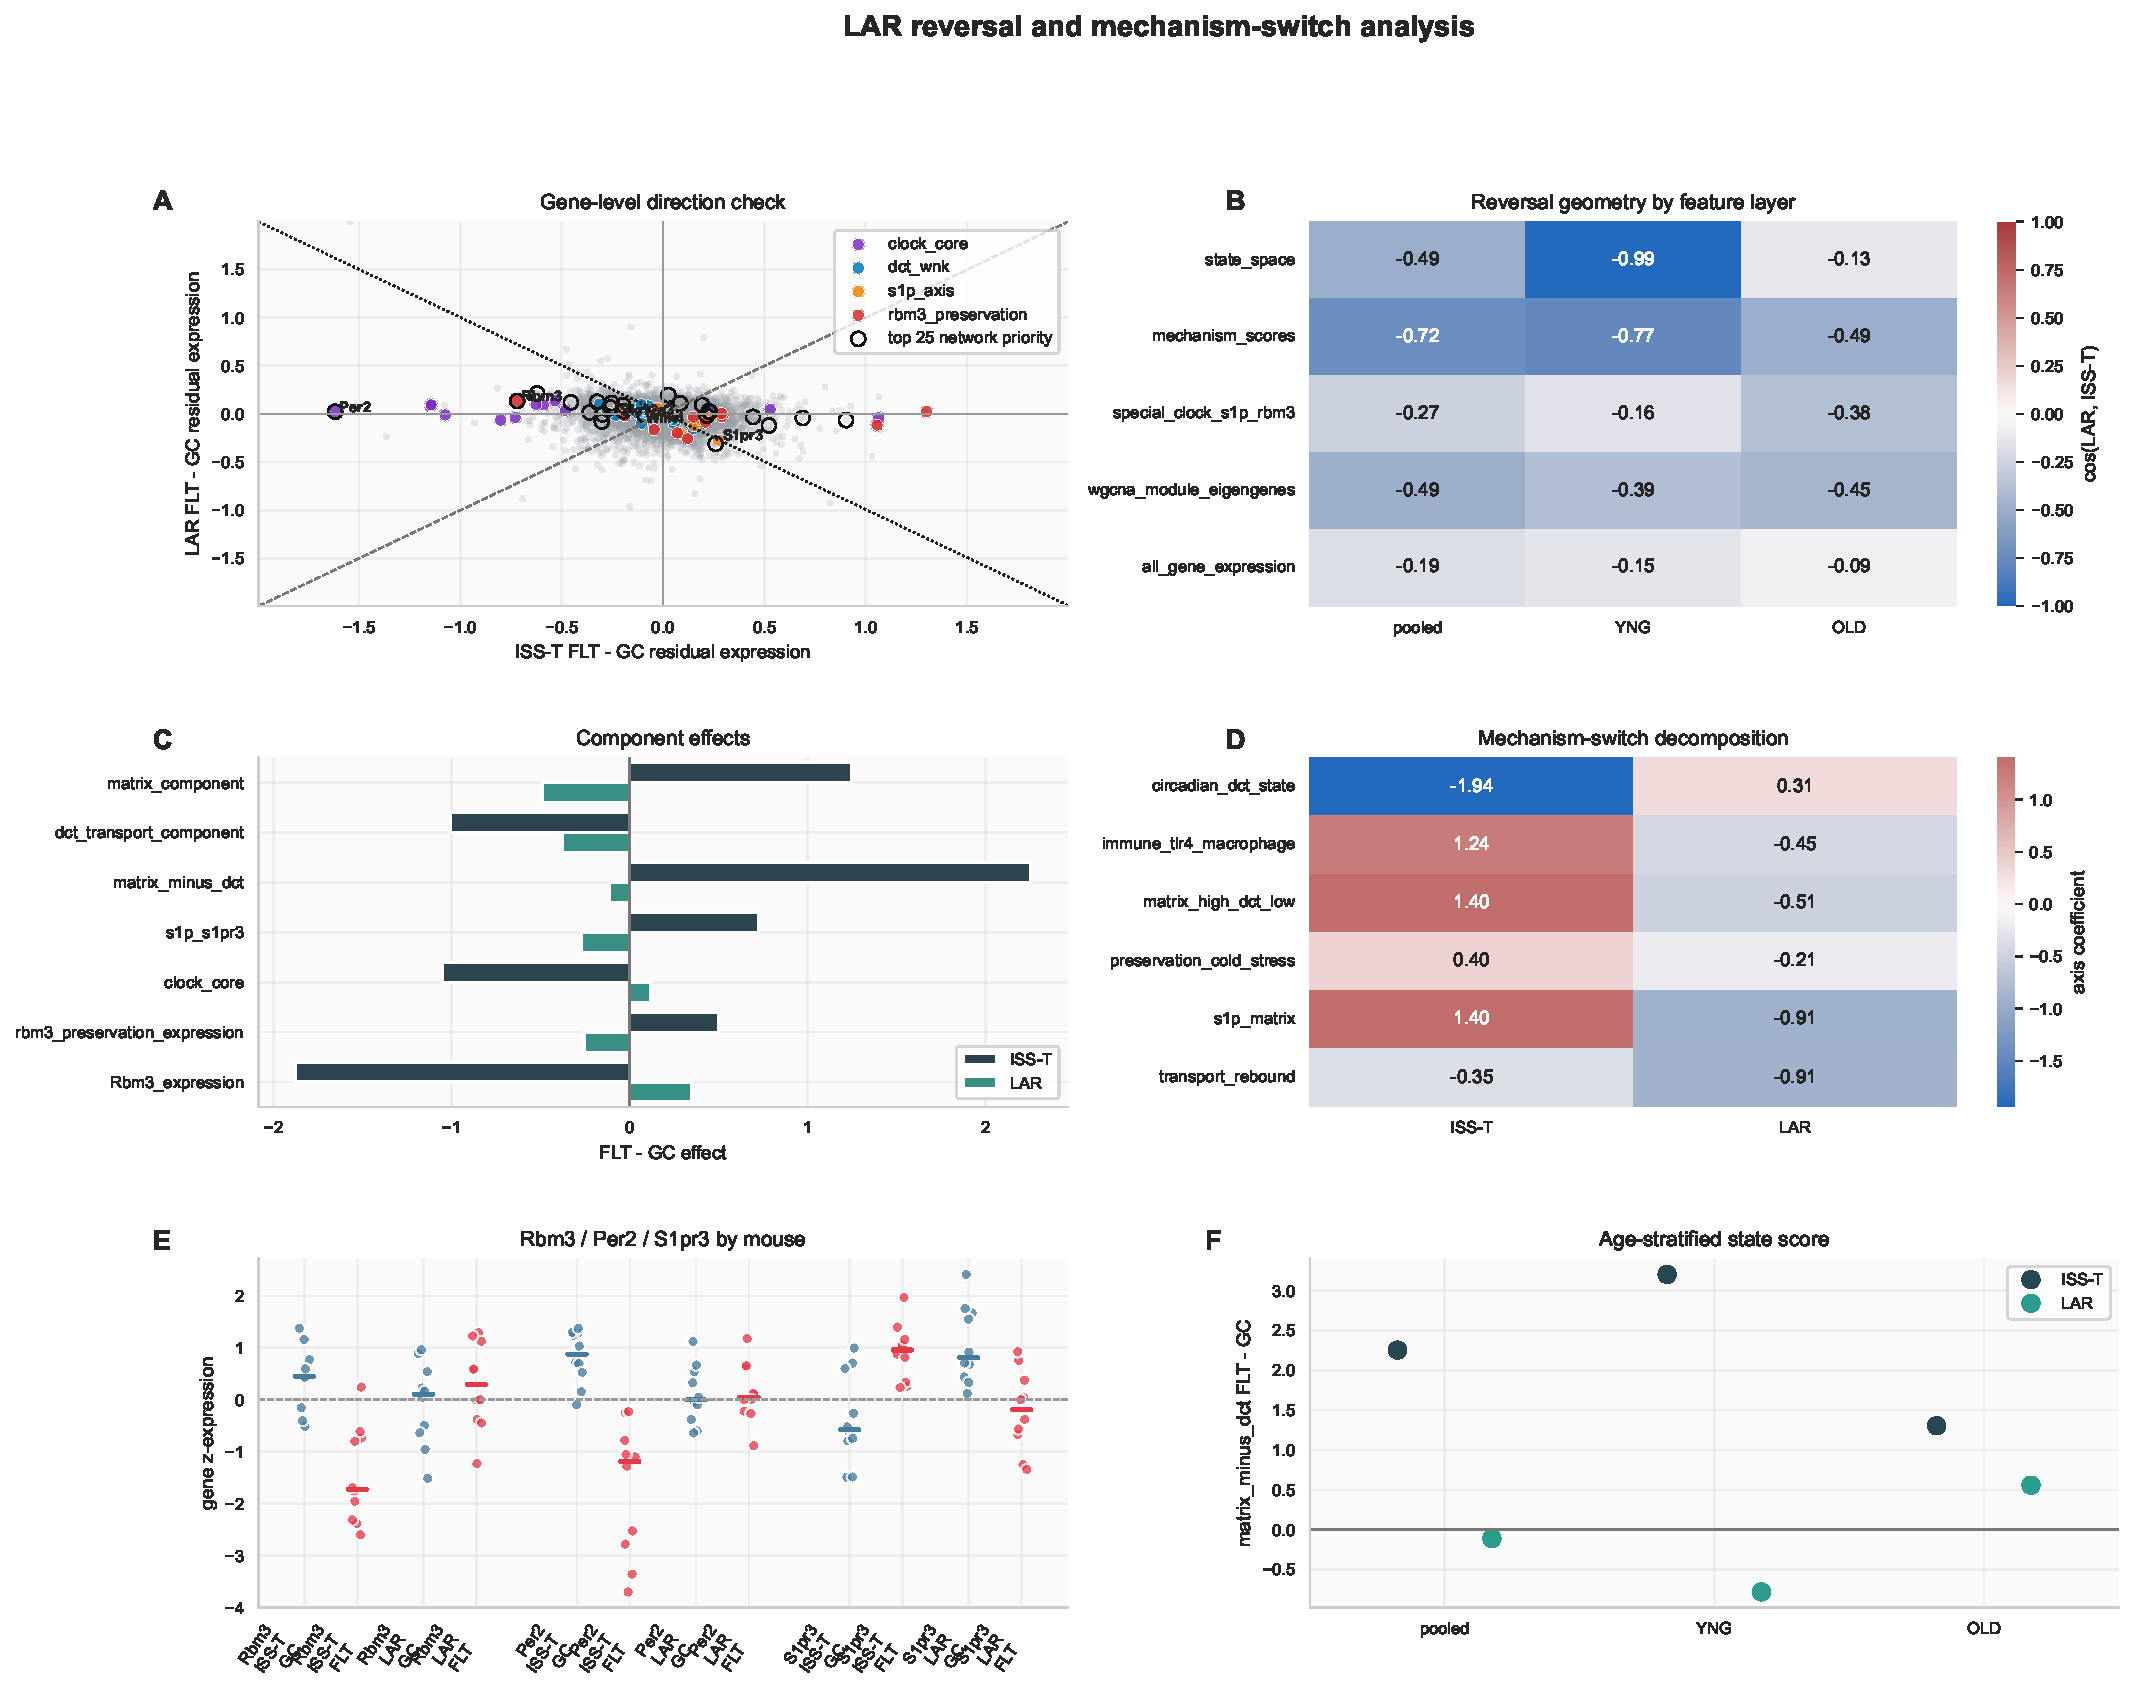
\includegraphics[width=\textwidth]{fig12_lar_reversal_dashboard.pdf}
\caption{\textbf{Live-return arm attenuation/divergence dashboard.} The young-LAR opposite point estimate is hypothesis-generating only; the LAR effect is not statistically distinguishable from zero.}
\end{figure}

\begin{figure}[H]
\centering
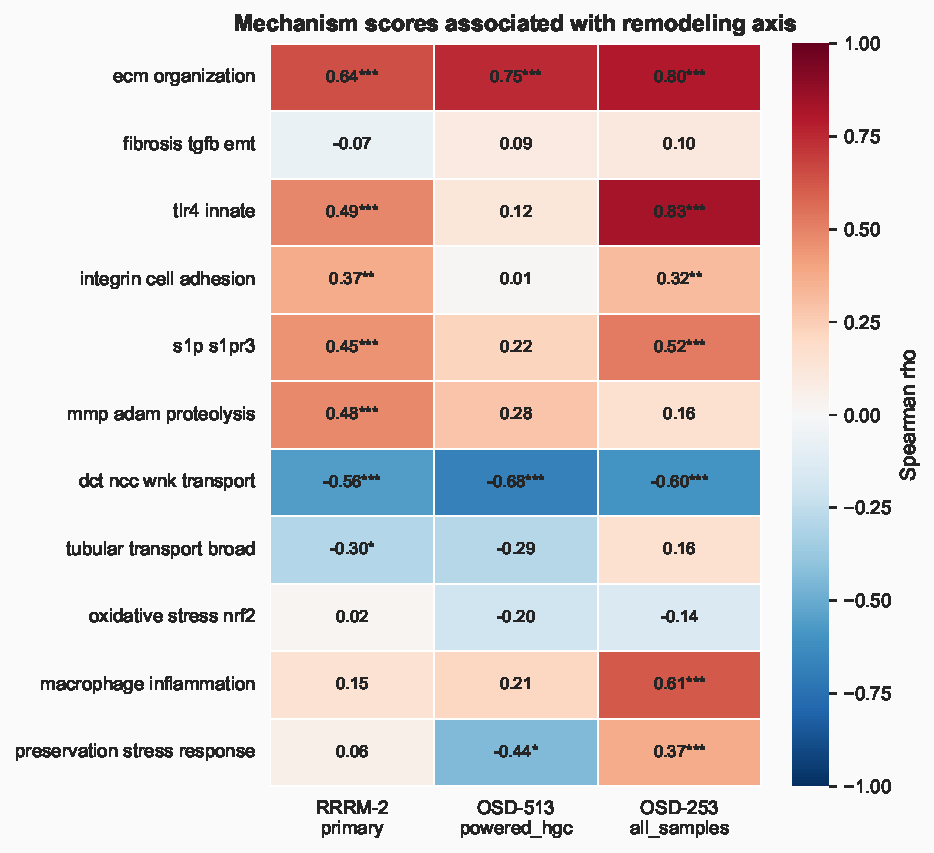
\includegraphics[width=0.82\textwidth]{fig6_mechanism_score_heatmap.pdf}
\caption{\textbf{Mechanism-score associations with the recurrent remodeling score} across RRRM-2, OSD-513, and OSD-253.}
\end{figure}

% =====================================================================
\section{Verification notes}

The following independent checks were performed on the OSD-462 anchor. (i) The eight \code{tests/test\_osd462\_anchor.py} unit tests pass. (ii) NCC phosphosite flight effects were re-derived directly from the raw \code{siteQuant\_360} workbook (log$_2$ of TMT signal-to-noise, 10 FL vs 10 GC channels, Welch $t$-test, no pipeline code): Thr53 $-0.99$, Thr65 $-0.93$ ($p=2.3\times10^{-6}$), Thr68 $-0.94$, Thr89 $-1.07$; non-regulatory Ser96/Ser120/Ser122 flat --- confirming the pipeline output in direction, magnitude, and significance. (iii) Total NCC protein flight effect ($+0.089$, 70 peptides) and the matrix-protein effects were confirmed from \code{protein\_effects\_gene\_anyplex.tsv}. (iv) The RNA recurrence cosine and leave-one-pathway-out range were reproduced from \code{osd462\_rna\_recurrence.tsv}. The site-specific pattern (regulatory cluster down, non-regulatory sites flat, total protein flat) is the principal internal control establishing that the phospho-axis result is genuine activating-site regulation rather than a normalization or abundance artifact.

\vspace{1em}
\noindent\itshape Supplement to Manuscript v8. The spaceflight NCC dephosphorylation phenotype confirmed here was first established by the Cosmic Kidney Disease study (Siew et al., \emph{Nature Communications}, 2024).

\end{document}
